\documentclass[a4paper,11pt]{kth-mag}
\usepackage[T1]{fontenc}
\usepackage{textcomp}
\usepackage{lmodern}
\usepackage[latin1]{inputenc}
\usepackage[swedish,english]{babel}
\usepackage{modifications}
\usepackage{hyperref}
\title{SimpleGraphPlotter v1.6}

\subtitle{}
\foreigntitle{}
\author{Jim Holmstr\"{o}m\\\href{mailto:jimho@kth.se}{jimho@kth.se}}
\date{\today}
\blurb{}

%\trita{TRITA xxx yyyy-nn}
\trita{}
\begin{document}
\frontmatter
\pagestyle{empty}
\removepagenumbers
\maketitle
\selectlanguage{english}
%\begin{abstract}
%  This is a skeleton for KTH theses. More documentation
%  regarding the KTH thesis class file can be found in
%  the package documentation.

%Lorem ipsum dolor sit amet, consectetuer adipiscing elit. Mauris
%purus. Fusce tempor. Nulla facilisi. Sed at turpis. Phasellus eu
%ipsum. Nam porttitor laoreet nulla. Phasellus massa massa, auctor
%rutrum, vehicula ut, porttitor a, massa. Pellentesque fringilla. Duis
%nibh risus, venenatis ac, tempor sed, vestibulum at, tellus. Class
%aptent taciti sociosqu ad litora torquent per conubia nostra, per
%inceptos hymenaeos.
%\end{abstract}
%\clearpage
%\begin{foreignabstract}{swedish}
%  Denna fil ger ett avhandlingsskelett.
%  Mer information om \LaTeX-mallen finns i
%  dokumentationen till paketet.

%Lorem ipsum dolor sit amet, consectetuer adipiscing elit. Mauris
%purus. Fusce tempor. Nulla facilisi. Sed at turpis. Phasellus eu
%ipsum. Nam porttitor laoreet nulla. Phasellus massa massa, auctor
%rutrum, vehicula ut, porttitor a, massa. Pellentesque fringilla. Duis
%nibh risus, venenatis ac, tempor sed, vestibulum at, tellus. Class
%aptent taciti sociosqu ad litora torquent per conubia nostra, per
%inceptos hymenaeos.
%\end{foreignabstract}
%\clearpage
\tableofcontents*
\mainmatter
\pagestyle{newchap}

\chapter{Introduction}
In the following part firstly the problem will be explained and secondly the requirements for a basic plotter will be enlisted.
A plotter is a program that can plot functions from strings which defines the functions by ordinary math syntax.

\section{Requirements}
A few basic things is needed to have a functioning math plotter. One must be able to:
\begin{enumerate}
    \item Define a function given ordinary math syntax.
    \item Parse the inputed function and plot it accordingly.
    \item Add/Remove functions from plotarea.
    \item The plotarea should be scrollable both vertical and horizontal.
    \item The range should be fixed to the unit-cube.\footnote{This restriction will be handled in section \ref{sec:scope}}
    \item Display the axis of the plot.
    \item The parser must be tested.

\end{enumerate}

\section{Scope}
\label{sec:scope}
The amount of functionallity that is possible to put in a system like this is almost endless so a few delimitations has to be made in order to complete the project.
The currently biggest restriction to the plotter is the lack of ability to zoom or change the range from the unit-cube.

\begin{figure}[ht]
    \begin{center}
        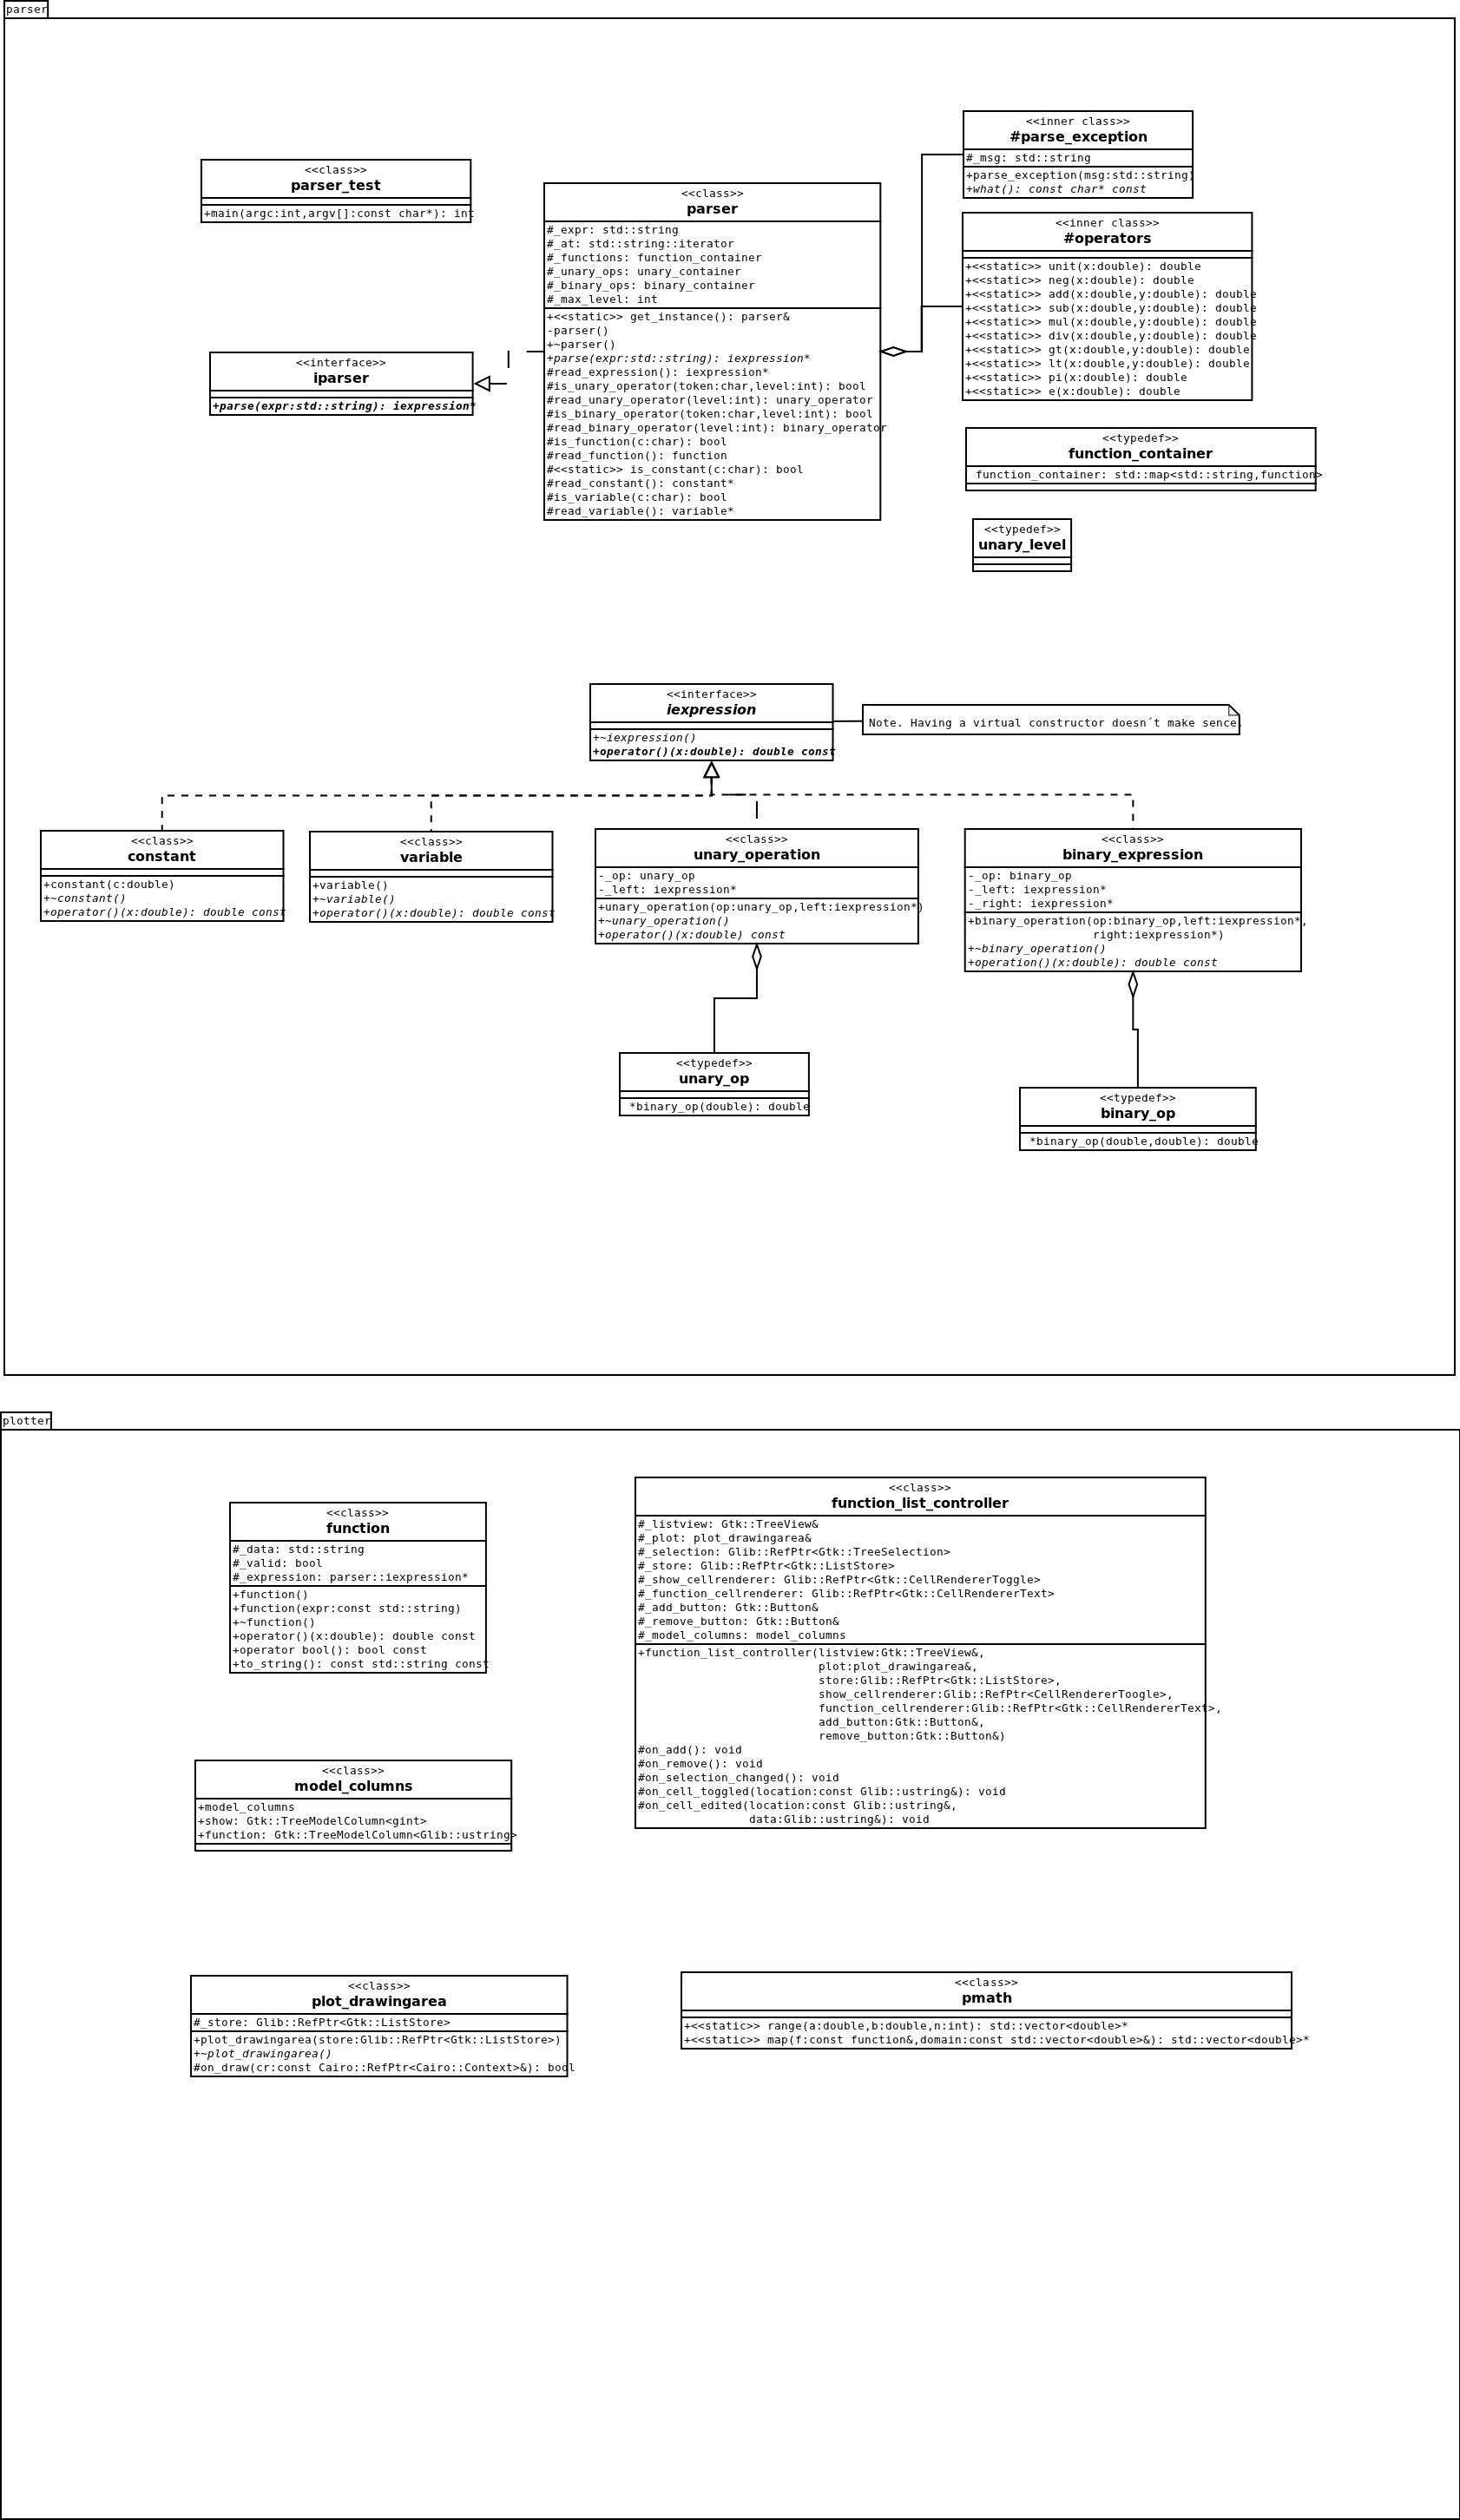
\includegraphics{uml.png}
        \caption{\small{An UML showing the structure and the enclosure.}}\label{fig:UML}
    \end{center}
\end{figure}

that we refer to here: \ref{RDF_4}
\end{document}
